\documentclass[10pt,a4paper]{article}
\usepackage[utf8]{inputenc}
\usepackage[T1]{fontenc}
\usepackage[margin=1.8cm,top=2.6cm,bottom=2.2cm]{geometry}
\usepackage{parskip}
\usepackage{microtype}
\usepackage{amsmath,amssymb,mathtools}
\usepackage{array,booktabs,tabularx,multirow}
\usepackage[table]{xcolor}
\usepackage{graphicx,float}
\usepackage{titlesec}
\usepackage{enumitem}
\usepackage{fancyhdr}
% ---- Section numbering: Roman numerals ---------------------------------
\renewcommand\thesection{\Roman{section}}
% ---- Equation numbering: (I.1), (II.2), etc. ---------------------------
\numberwithin{equation}{section}

% ---- Section formatting ------------------------------------------------
\titleformat{\section}{\large\bfseries}{\thesection.\;}{0em}{}[\titlerule]
\titleformat{\subsection}{\normalsize\bfseries}{}{0em}{}
\titleformat{\subsubsection}{\normalsize\itshape}{}{0em}{}
\titlespacing{\section}{0pt}{1.6ex plus .2ex}{0.6ex}
\titlespacing{\subsection}{0pt}{1.0ex}{0.3ex}

% ---- Page headers ------------------------------------------------------
\pagestyle{fancy}
\fancyhf{}
\setlength{\headheight}{15pt}
\fancyhead[L]{\small\textit{SWV Forward Model}}
\fancyhead[R]{\small Aaran Nihalani $\bullet$ Eton iGEM Dry Lab}
\fancyfoot[C]{\small\thepage}
\renewcommand{\headrulewidth}{0.35pt}

% ---- Key result box (left rule, shaded) --------------------------------
\newenvironment{keyresult}{%
  \par\addvspace{0.5ex}%
  \setlength{\fboxsep}{6pt}%
  \noindent\colorbox{black!6}\bgroup
  \minipage{\dimexpr\linewidth-2\fboxsep}%
  \small
}{%
  \endminipage\egroup\par\addvspace{0.5ex}%
}

% ---- Macros ------------------------------------------------------------
\newcommand{\cit}[1]{[#1]}
\newcommand{\Fk}{F_k}
\newcommand{\kET}{k_{\text{ET}}}
\newcommand{\kref}{k_{\text{ref}}}
\newcommand{\betaD}{\beta}
\newcommand{\Gtot}{\Gamma_{\text{tot}}}
\newcommand{\Geq}{\Gamma_{\text{eq}}}
\newcommand{\Gred}{\Gamma_{\text{red}}}
\newcommand{\Gox}{\Gamma_{\text{ox}}}
\newcommand{\Esw}{E_{\text{sw}}}
\newcommand{\kzero}{k_0}
\newcommand{\Pd}{P(d)}
% \kappa already defined by amsmath
\newcommand{\DI}{\Delta I}
\newcommand{\nm}{\,\text{nm}}
\newcommand{\Ang}{\,\text{\AA}}
\newcommand{\FLAG}{\textbf{[FLAG: unconfirmed]}}
\newcommand{\says}[1]{\par\noindent\textit{\small $\triangleright$\;#1}\par\smallskip}

\begin{document}

%=======================================================================
\begin{center}
{\LARGE\bfseries SWV Forward Model}\\[0.4em]
{\large From Cleavage Fraction to Recorded Voltammogram}\\[0.25em]
{\small\color{gray} Eton iGEM 2026, Dry Lab \quad$|$\quad
Synthesis of Layers 6, 8, 9, 10, 11, 13 \quad$|$\quad
\texttt{swv\_forward\_model.py}}
\end{center}
\vspace{0.4em}\hrule\vspace{0.7em}

%=======================================================================
\section{What This Model Does}
\label{sec:overview}

\subsection{The physical story}

Picture the electrode surface. Thousands of peptide chains are chemisorbed to a gold
disc through a short alkyl spacer. Each chain ends in a methylene blue (MB) dye
molecule. MB is a redox reporter: it can gain or lose electrons, and we detect that
electrochemically. MMP-9, if present in the wound fluid, cuts each peptide at a
specific bond. The MB label falls away. The electrochemical signal drops.

The SWV forward model answers one question precisely: \textbf{if a fraction $\Fk$
of those peptide chains have been cleaved, what voltammogram would we actually
record?}

Answering this requires three pieces of physics, linked in sequence:

\begin{enumerate}[leftmargin=*,noitemsep]
  \item \textbf{Tether geometry.} MB is not at a fixed distance from the gold
    surface. The peptide chain is flexible and wiggles thermally, so MB samples a
    range of distances. We need the probability distribution $P(d)$ of those
    distances, because the electron transfer rate depends exponentially on $d$.

  \item \textbf{Electron transfer kinetics.} Once we know $d$, we can calculate how
    fast the redox reaction is. This rate $k_0(d)$ sets how MB responds to the SWV
    voltage waveform.

  \item \textbf{BV-SWV simulator.} Given the rate $k_0$, a Butler--Volmer model
    converts the SWV waveform into the net current $\DI(E)$ that the potentiostat
    records. Averaging over the $P(d)$ distribution and scaling by $(1 - \Fk)$
    gives the complete voltammogram.
\end{enumerate}

\noindent The chain is therefore:
\[
  [\text{MMP-9}],\;t
  \;\xrightarrow{\text{kinetics (Sec.~VII)}}\; \Fk
  \;\xrightarrow{\text{tether + ET (Sec.~II--III)}}\; k_0(d),\;P(d)
  \;\xrightarrow{\text{BV-SWV (Sec.~IV--V)}}\; \DI(E)
\]

\subsection{How to read this report}

Each section opens with the physical picture, then derives the equations that
formalise it, and closes with a \textbf{Key result} box. Every equation is
followed by a plain-English gloss beginning with \textit{This says.} Parameters
are tabulated at the section where they first appear. The code implementing
all steps is in \texttt{swv\_forward\_model.py}.

All parameter values are confirmed from papers physically present in
\texttt{papers/swv\_forward\_model/} or cross-referenced from other layer paper
folders as noted. Values that remain unconfirmed are labelled \FLAG{}.

%=======================================================================
\section{Tether Geometry: Where Does MB Sit?}
\label{sec:pd}

\subsection{Physical picture}

The gold electrode surface is coated with a mixed self-assembled monolayer (SAM).
The active component is our peptide probe: a C6 alkyl spacer anchors to the gold
via a thiol group, and the ten-residue peptide SGKIPRTLTA extends away from the
surface, with MB attached at the far end. The ``background'' component is
6-mercaptohexanol (MCH), which passivates the surface and prevents non-specific
binding.

At body temperature in wound fluid, the peptide chain is flexible. Rather than
sitting at a fixed distance, MB thermally fluctuates across a range of distances
from the gold surface. Figure~\ref{fig:valid}C shows this: $P(d)$ is the probability
density of finding MB at distance $d$ from the gold.

\textbf{Why does this matter?} Because electron transfer probability falls
exponentially with distance. A probe with MB 10~\AA\ from the gold has a rate
orders of magnitude higher than one with MB at 25~\AA. The voltammogram is the
average over all these probes, and that average is dominated by the shape of $P(d)$.

\subsection{Freely jointed chain (FJC) model}

We model the peptide as a \textbf{freely jointed chain}: $N_K$ rigid segments of
length $b$ joined at random orientations, like links in a necklace. This is the
simplest polymer model that captures the key physics of an unstructured flexible
chain. More elaborate models (worm-like chain, all-atom MD) are listed in
Section~\ref{sec:limits} as future work.

\begin{center}
\begin{tabular}{@{}llll@{}}
\toprule
\textbf{Parameter} & \textbf{Symbol} & \textbf{Value} & \textbf{Source} \\
\midrule
Residue count & $N_{\text{res}}$ & 10 & SGKIPRTLTA \\
Contour length per residue & $\ell_0$ & 0.38 nm & standard \\
Kuhn length & $b$ & 0.76 nm & Kohn 2004~\cit{2} \\
C6 linker length & $d_{\text{C6}}$ & 0.756 nm & \cit{1} Fig.~4 \\
\bottomrule
\end{tabular}
\end{center}

\vspace{0.5em}
Since each Kuhn segment spans two residues ($b = 2\ell_0$), the number of Kuhn
segments in the ten-residue peptide is $N_K = N_{\text{res}} / 2 = 5$.

The mean-squared end-to-end distance of the chain:
\begin{equation}
  \langle r^2 \rangle = N_K\, b^2 = 5 \times (0.76)^2 = 2.888\;\text{nm}^2
  \label{eq:r2}
\end{equation}
\says{a longer or stiffer chain (larger $N_K b^2$) pushes MB farther from the surface on average.}

Because the chain is isotropic, the three spatial directions ($x$, $y$, $z$) are
equivalent. The standard deviation of MB distance along the surface-normal axis
($z$, pointing away from gold) is:
\begin{equation}
  \sigma_z = \sqrt{\langle r^2 \rangle / 3} = \sqrt{2.888/3} = 0.981\;\text{nm}
  \label{eq:sigmaz}
\end{equation}
\says{$\sigma_z$ is the typical spread of MB positions above the surface. It is roughly 1~nm, comparable to the C6 linker length itself.}

\subsection{The distance distribution $P(d)$}

The surface is a hard wall: MB cannot go below $d = d_{\text{C6}}$ (the linker
holds it there). Above that, the chain end-position follows a 3D Gaussian, conditioned
on $z \geq 0$ and shifted by $d_{\text{C6}}$. This gives a half-Gaussian:
\begin{equation}
  P(d) = \frac{\sqrt{2/\pi}}{\sigma_z}
         \exp\!\left(-\frac{(d - d_{\text{C6}})^2}{2\sigma_z^2}\right),
         \qquad d \geq d_{\text{C6}}
  \label{eq:Pd}
\end{equation}
\says{the most likely position for MB is just above the linker tip; it becomes progressively less likely farther away, with spread $\sigma_z \approx 1$~nm.}

The mean distance (centre of mass of the distribution):
\begin{equation}
  \langle d \rangle = d_{\text{C6}} + \sigma_z\sqrt{2/\pi}
  = 0.756 + 0.784 = 1.540\;\text{nm} = 15.4\Ang
  \label{eq:dmean}
\end{equation}

\begin{keyresult}
\textbf{Key result:} MB sits at a mean distance of 15.4~\AA\ from the gold surface,
with a spread of 9.8~\AA\ ($\sigma_z$). The distribution peaks at the linker tip (7.56~\AA)
and has a long tail to larger distances. See Figure~\ref{fig:valid}C.
\end{keyresult}

%=======================================================================
\section{Electron Transfer Kinetics: How Fast Does MB React?}
\label{sec:ket}

\subsection{Physical picture}

For MB to undergo redox chemistry, an electron must tunnel through the molecular
bridge between the electrode and MB. Tunnelling probability falls off exponentially
with distance: every extra \AA ngstr\"{o}m makes tunnelling roughly $e^{-1} = 37$\%
as likely. This means the electron transfer rate $k_0$ is extremely sensitive to
exactly where MB sits, which is why the $P(d)$ distribution calculated above
matters so much.

The tunnelling rate also depends on the medium: electrons tunnel faster through
conjugated aromatic systems than through saturated alkyl chains. The C6 linker
plus peptide backbone here is effectively an insulating alkyl bridge, so the
decay is rapid.

\subsection{Tunnelling decay equation}

\begin{center}
\begin{tabular}{@{}llll@{}}
\toprule
\textbf{Parameter} & \textbf{Symbol} & \textbf{Value} & \textbf{Source} \\
\midrule
Tunnelling decay constant & $\beta$ & 1.0~\AA$^{-1}$ & Smalley 1995~\cit{3} \\
Rate at C6 tip & $k_{\text{ref}}$ & $7.8\times10^4$~s$^{-1}$ & \cit{1} Fig.~3 \\
\bottomrule
\end{tabular}
\end{center}

The rate at any distance $d$ beyond the C6 linker tip:
\begin{equation}
  k_0(d) = k_{\text{ref}} \exp\!\bigl(-\beta (d - d_{\text{C6}})\bigr)
  \label{eq:kETd}
\end{equation}
\says{each additional \AA ngstr\"{o}m of distance reduces the rate by a factor $e^{-1.0} = 0.37$, i.e.\ a 63\% reduction per \AA ngstr\"{o}m.}

At the mean label distance $\langle d \rangle = 15.4$~\AA:
\begin{equation}
  k_0(\langle d \rangle) = 7.8\times10^4 \times \exp\!\bigl(-1.0 \times (15.4 - 7.56)\bigr)
  = 7.8\times10^4 \times e^{-7.84} = 31\;\text{s}^{-1}
  \label{eq:kETmean}
\end{equation}

This is a drop of more than 2000-fold from the linker tip to the mean position. The
rate would be $k_{\text{ref}} = 7.8\times10^4$~s$^{-1}$ if the peptide were absent
(MB sitting right on the C6 tip), but the 7.84~\AA\ of extra chain drops it to
31~s$^{-1}$. Probes with MB closer than average contribute disproportionately more
current (faster rate), which is why we must integrate over $P(d)$ rather than just
use the mean.

\subsection{The dimensionless kinetic parameter $\kappa$}

\textbf{Whether MB responds measurably to the SWV waveform depends not on $k_0$
alone, but on how fast it is relative to the SWV pulse duration.} This comparison
is captured by the dimensionless parameter:
\begin{equation}
  \kappa = k_0 \times \tau = \frac{k_0}{2f}
  \label{eq:kappa}
\end{equation}
\says{$\kappa$ is the number of redox events that can happen during one SWV half-pulse of duration $\tau = 1/(2f)$.}

There are three regimes:
\begin{itemize}[noitemsep,leftmargin=*]
  \item $\kappa \gg 1$ (reversible): the reaction equilibrates fully during the pulse.
    Net current $\DI \to 0$ because no charge accumulates between pulses. Sensitivity is low.
  \item $\kappa \ll 1$ (irreversible): the reaction barely starts during the pulse.
    Net current again small. Sensitivity is low.
  \item $\kappa \approx 1$ (quasi-reversible): the reaction partially equilibrates.
    This is where $\DI$ is maximised and most sensitive to changes in $k_0$.
\end{itemize}

At our operating frequency $f = 15$~Hz and mean $k_0 = 31$~s$^{-1}$:
\begin{equation}
  \kappa_{\text{mean}} = \frac{31}{2 \times 15} = 1.04
  \label{eq:kappa_val}
\end{equation}

This is not a coincidence. The 15~Hz frequency was chosen precisely to sit at
$\kappa \approx 1$ for our peptide system, maximising sensitivity to cleavage.
The Fc internal reference electrode operates at $\kappa_{\text{Fc}} = 9{,}000$
(firmly reversible), which is required for a stable reference.

\begin{keyresult}
\textbf{Key result:} $k_0$ at the mean MB distance is 31~s$^{-1}$. At 15~Hz this
gives $\kappa = 1.04$, the quasi-reversible optimum for maximum sensitivity. Probes
closer to the gold have higher $k_0$ and higher $\kappa$; probes farther away have lower
$k_0$ and lower $\kappa$.
\end{keyresult}

%=======================================================================
\section{The BV-SWV Simulator: Waveform to Current}
\label{sec:bvsim}

\subsection{What SWV does}

Square-wave voltammetry (SWV) applies a voltage that steps along a staircase, with
a square pulse superimposed at each step. At each staircase potential $E_n$, the
voltage toggles between $E_n + \Esw$ (forward half-pulse) and $E_n - \Esw$
(backward half-pulse), each lasting $\tau = 1/(2f)$ seconds. The key measurement
is the \textbf{difference} in current at the end of each forward and backward
half-pulse:
\[
  \DI(E_n) = I_{\text{forward}} - I_{\text{backward}}
\]
Subtracting the two half-pulses cancels the background (capacitive) current and
doubles the faradaic (redox) signal. The result is a peak-shaped voltammogram
centred at the formal potential $E^{\circ\prime}$ of MB.

\subsection{The ODE governing surface coverage}

\begin{center}
\begin{tabular}{@{}llll@{}}
\toprule
\textbf{Parameter} & \textbf{Symbol} & \textbf{Value} & \textbf{Source} \\
\midrule
Transfer coefficient & $\alpha$ & 0.37 & \cit{1} Table~1 \\
Electron count & $n$ & 2 & Baker 2006~\cit{6} \\
Formal potential (MB) & $E^{\circ\prime}$ & $-0.250$~V vs.\ Ag/AgCl & \cit{6} \\
Probe surface density & $\Gtot$ & $3\times10^{-12}$~mol~cm$^{-2}$ & \cit{5} \\
Electrode area & $A$ & 0.0177~cm$^2$ & 1.5~mm disc \\
\bottomrule
\end{tabular}
\end{center}

During each half-pulse, the fraction of MB that is in the reduced form
($\Gred$, mol~cm$^{-2}$) evolves according to a first-order ODE:
\begin{equation}
  \frac{d\Gred}{dt} = k_f \Gox - k_b \Gred
  \label{eq:ode}
\end{equation}
\says{reduction (rate $k_f$) increases $\Gred$; oxidation (rate $k_b$) decreases it. $\Gox = \Gtot - \Gred$ is the oxidised fraction.}

The rates $k_f$ and $k_b$ depend on the applied potential through the
Butler--Volmer equations:
\begin{align}
  k_f(E) &= k_0 \exp\!\Bigl(-\frac{\alpha n F (E - E^{\circ\prime})}{RT}\Bigr)
  \label{eq:kf}\\[4pt]
  k_b(E) &= k_0 \exp\!\Bigl(\frac{(1-\alpha) n F (E - E^{\circ\prime})}{RT}\Bigr)
  \label{eq:kb}
\end{align}
\says{At $E \ll E^{\circ\prime}$, $k_f \gg k_b$: reduction is fast and MB is fully reduced. At $E \gg E^{\circ\prime}$, $k_b \gg k_f$: MB is fully oxidised. The peak current arises in between, around $E^{\circ\prime}$.}

\subsection{Exact solution for each half-pulse}

Because Eq.~(\ref{eq:ode}) is linear in $\Gred$, it has an exact analytical
solution over one half-pulse of duration $\tau$, starting from initial coverage
$\Gred^{(0)}$:
\begin{equation}
  \Gred(\tau) = \Geq + \bigl(\Gred^{(0)} - \Geq\bigr)\,e^{-(k_f+k_b)\tau}
  \label{eq:Gred_soln}
\end{equation}
\says{coverage relaxes exponentially toward the equilibrium value $\Geq$. The exponential decay constant $(k_f+k_b)\tau = \kappa$ sets how far it gets in time $\tau$.}

where the equilibrium reduced coverage is:
\begin{equation}
  \Geq = \frac{k_f}{k_f + k_b}\,\Gtot
  \label{eq:Geq}
\end{equation}
\says{at $E = E^{\circ\prime}$, $k_f = k_b$ so $\Geq = \Gtot/2$ (half reduced, half oxidised). Far from $E^{\circ\prime}$, one of $k_f, k_b$ dominates and $\Geq$ goes to 0 or $\Gtot$.}

The exponent $(k_f + k_b)\tau$ is precisely $\kappa$. When $\kappa \gg 1$, the
exponential $e^{-\kappa} \to 0$ and coverage fully reaches $\Geq$ during the pulse.
When $\kappa \ll 1$, the exponential $\approx 1$ and almost no change occurs.

\subsection{Sampled current and net $\DI$}

The anodic current sampled at the end of each half-pulse:
\begin{equation}
  I = nFA\bigl(k_b\,\Gred(\tau) - k_f\,\Gox(\tau)\bigr)
  \label{eq:Ianodic}
\end{equation}
\says{current is positive (anodic) when oxidation dominates. At equilibrium, $k_b \Gred = k_f \Gox$ exactly and $I = 0$. Current flows because the coverage has not fully relaxed to $\Geq$ by time $\tau$.}

The forward and backward half-pulses are chained across the staircase: the
coverage at the end of the forward pulse becomes the starting coverage for the
backward pulse, and so on. The simulator runs a 5-pulse burn-in at the starting
potential before scanning to ensure periodic steady state.

Figure~\ref{fig:valid}A shows a unit test: the simulator run at $\kappa = 10$
produces a peak with FWHM = 60.6~mV, within the expected 40--90~mV range for
$n = 2$, $\Esw = 25$~mV.

\begin{keyresult}
\textbf{Key result:} The BV-SWV simulator converts $k_0$ and applied potential $E$
into a current sample in one analytical step (no numerical ODE integration needed).
Each half-pulse has an exact closed-form solution (Eq.~\ref{eq:Gred_soln}).
The sensitivity to $k_0$ is maximal near $\kappa = 1$, which is where our peptide
system operates.
\end{keyresult}

%=======================================================================
\section{Distance-Averaged Voltammogram: Combining $P(d)$ and $\DI$}
\label{sec:avg}

\subsection{Physical picture}

We now have $P(d)$ (Section~II) and know how to compute $\DI$ for any $k_0$
(Sections~III--IV). The measured voltammogram is the sum over \emph{all} probes,
each at its own distance $d$, each contributing its own current.

Critically, probes with MB very close to the gold (small $d$, large $k_0$, large
$\kappa$) are in the reversible limit and contribute \emph{almost no} net current.
Probes near the mean distance ($d \approx 15.4$~\AA, $\kappa \approx 1$) dominate
the signal. This makes the measured voltammogram shape robust: even if a few probes
sit unusually close to the gold, they do not dominate.

\subsection{The averaging integral}

After cleavage fraction $\Fk$ of probes have lost their MB label, only the remaining
$(1 - \Fk)$ fraction contribute current. The total voltammogram:
\begin{equation}
  \DI(E;\,\Fk) = (1-\Fk)\,\Gtot\,A
    \int_{d_{\text{C6}}}^{\infty} P(d)\;\DI_{\text{norm}}\!\bigl(E;\,k_0(d)\bigr)\;dd
  \label{eq:DI_avg}
\end{equation}
\says{the measured current is $(1-\Fk)$ times the integral over all probe distances. Each distance contributes proportionally to how many probes sit there [$P(d)$] and how much current each generates [$\DI_{\text{norm}}(E;\,k_0(d))$].}

This is the \textbf{central equation of the model}. It connects the biological
input ($\Fk$) to the electrochemical output ($\DI(E)$) through two layers of
physics: the tether geometry $P(d)$ and the ET kinetics $k_0(d)$.

The $(1-\Fk)$ factor is exact when cleavage is binary (each probe is either fully
intact or fully cleaved). This is a good approximation because MMP-9 cleaves the
Arg|Thr bond stoichiometrically, and the remaining C6-thiol stub has no MB label.

\subsection{Numerical implementation}

The integral in Eq.~(\ref{eq:DI_avg}) is evaluated over 80 distance points
spanning $d_{\text{C6}}$ to $d_{\text{C6}} + 5\sigma_z$. At each point, the
BV-SWV simulation runs the pulse chain described in Section~IV. Gauss quadrature
over 80 points is sufficient because $P(d)$ is smooth and the integrand varies
smoothly with $d$.

Figure~\ref{fig:calib}A shows the resulting voltammograms for six values of
$\Fk$: 0, 0.2, 0.4, 0.6, 0.8, and 0.95. The peak shrinks proportionally
with $(1 - \Fk)$ while the peak position and width stay constant.

\begin{keyresult}
\textbf{Key result:} Cleavage reduces the peak area by exactly $(1 - \Fk)$ and
leaves the peak shape (position, FWHM) unchanged. This is the foundation of the
calibration in Section~VI.
\end{keyresult}

%=======================================================================
\section{Calibration: Reading $\Fk$ from the Voltammogram}
\label{sec:calib}

\subsection{Extracting the peak area}

The voltammogram $\DI(E;\,\Fk)$ is well described by a Gaussian in potential:
\begin{equation}
  \DI_{\text{fit}}(E) = A_{\text{peak}}
    \exp\!\Bigl(-\frac{(E - E_{\text{peak}})^2}{2\sigma_E^2}\Bigr)
  \label{eq:gauss}
\end{equation}
The integrated area $A_{\text{area}} = A_{\text{peak}}\,\sigma_E\sqrt{2\pi}$ (in
A$\cdot$V) is more reproducible than peak height alone because it is insensitive
to small shifts in $E_{\text{peak}}$ or FWHM across electrodes.

\subsection{Calibration equation}

Because the voltammogram amplitude is proportional to $(1-\Fk)$ (Eq.~\ref{eq:DI_avg}),
the calibration is linear. The cleavage fraction is recovered by:
\begin{equation}
  \Fk = 1 - \frac{A_{\text{area}}(\text{after})}{A_{\text{area}}(\text{before})}
  \label{eq:Fk_recovery}
\end{equation}
\says{the fractional drop in peak area equals the fraction of probes cleaved. A 30\% drop means 30\% of probes were cut.}

Figure~\ref{fig:calib}B confirms this: the maximum deviation from linearity across
$\Fk \in [0, 0.95]$ is only 2\%, confirming that Eq.~(\ref{eq:Fk_recovery}) is
the correct readout equation.

Figure~\ref{fig:calib}C confirms that the peak position $E_{\text{peak}}$ and FWHM
do not drift with $\Fk$ (variation $<$ 3~mV). If these were shifting significantly,
it would indicate non-binary cleavage behaviour or surface artefacts.

\begin{keyresult}
\textbf{Key result:} $A_{\text{area}}$ is linear in $(1 - \Fk)$ to within 2\%.
Reading $\Fk$ from the voltammogram requires only the ratio of peak areas
before and after incubation.
\end{keyresult}

%=======================================================================
\section{Ferrocene Reference: Correcting for Surface Variability}
\label{sec:ratio}

\subsection{The problem}

The absolute MB peak area varies $\pm$15\% between electrodes because SAM deposition
is not perfectly reproducible. Without correction, this electrode-to-electrode
variability would mask the cleavage signal. For example, a 15\% drop in area due
to a poorly formed SAM looks identical to a 15\% drop due to cleavage.

\subsection{The solution: an internal reference}

Ferrocene (Fc) is co-deposited on the same electrode as a reference molecule. Fc
is structurally simple, electrochemically stable, and completely insensitive to
MMP-9 (it is not a peptide). Its peak area $A_{\text{Fc}}$ tracks the same SAM
variability as MB but does not change when protease is added. Therefore, the ratio
$A_{\text{MB}} / A_{\text{Fc}}$ cancels the common variability.

\begin{center}
\begin{tabular}{@{}llll@{}}
\toprule
\textbf{Parameter} & \textbf{Symbol} & \textbf{Value} & \textbf{Source} \\
\midrule
Fc transfer rate & $k_{0,\text{Fc}}$ & $2.7\times10^5$~s$^{-1}$ & \cit{1} Fig.~3 \\
Fc formal potential & $E^{\circ\prime}_{\text{Fc}}$ & $+0.210$~V vs.\ Ag/AgCl & \cit{1} \\
Fc $\kappa$ at 15~Hz & $\kappa_{\text{Fc}}$ & 9000 (reversible) & calculated \\
\bottomrule
\end{tabular}
\end{center}

The ratiometric signal, normalised to its value before protease addition:
\begin{equation}
  \rho(t) = \frac{R(t)}{R(0)}, \qquad R(t) = \frac{A_{\text{MB}}(t)}{A_{\text{Fc}}(t)}
  \label{eq:rho}
\end{equation}
\says{$\rho = 1$ when no probes are cleaved; $\rho < 1$ after cleavage reduces the MB signal. The Fc signal appears in both $R(t)$ and $R(0)$ and cancels out, removing surface drift.}

The recovered cleavage fraction:
\begin{equation}
  \Fk(t) = 1 - \rho(t)
  \label{eq:Fk_rho}
\end{equation}
\says{a 20\% drop in $\rho$ means 20\% of probes were cleaved. This follows from Eq.~(\ref{eq:Fk_recovery}) with Fc providing the drift reference.}

Because $\kappa_{\text{Fc}} = 9000 \gg 1$, the Fc peak is in the fully reversible
regime: its area is insensitive to $k_{0,\text{Fc}}$ variations and frequency
changes, making it a stable reference. White and Plaxco (2010)~\cit{7} confirmed
that this ratiometric approach suppresses drift by two orders of magnitude in
electrochemical aptamer sensors.

Figure~\ref{fig:ratio} shows the Fc voltammogram and confirms that the recovered
$\Fk$ matches the true $\Fk$ to within 3.4\% across the full range.

\begin{keyresult}
\textbf{Key result:} Ratiometric correction with Fc reduces electrode-to-electrode
variability from $\pm$15\% to $<$3.4\%, enabling detection of cleavage fractions
down to $\sim$10\%.
\end{keyresult}

%=======================================================================
\section{From MMP-9 Concentration to Voltammogram}
\label{sec:concmap}

\subsection{Kinetic link: concentration to cleavage fraction}

Given a free MMP-9 concentration and an incubation time, the cleavage fraction
follows from pseudo-first-order kinetics:
\begin{equation}
  \Fk(t) = 1 - \exp\!\bigl(-k_{\text{eff,surf}}\,[\text{MMP-9}]\,t\bigr)
  \label{eq:Fk_kinetics}
\end{equation}
\says{$\Fk$ starts at zero (no probes cleaved) and rises toward 1 as more probes are cut. It rises faster at higher MMP-9 concentration and with longer incubation.}

This is the exact solution to the first-order cleavage ODE: the rate at which intact
probes are cut is proportional to the MMP-9 concentration and to how many intact
probes remain. ``Pseudo-first-order'' means we treat [MMP-9] as constant throughout
the incubation, which is valid when enzyme concentration ($\geq$6~nM) is much larger
than the surface peptide density ($\approx$10~pM at $\Gtot = 3\times10^{-12}$~mol~cm$^{-2}$,
0.0177~cm$^2$ electrode).

\begin{center}
\begin{tabular}{@{}llll@{}}
\toprule
\textbf{Parameter} & \textbf{Symbol} & \textbf{Value} & \textbf{Source} \\
\midrule
Solution $k_{\text{cat}}/K_m$ & --- & 67{,}500~M$^{-1}$s$^{-1}$ & Kridel 2001~\cit{4} \\
Surface correction & $\eta$ & 0.20 & Layer 8 \FLAG \\
Effective surface rate & $k_{\text{eff,surf}}$ & 13{,}500~M$^{-1}$s$^{-1}$ & derived \\
\bottomrule
\end{tabular}
\end{center}

The surface correction factor $\eta$ accounts for the fact that peptides on a
surface are oriented, crowded, and partly blocked by the MCH background. The
central estimate is $\eta = 0.20$ (20\% of solution activity). This is the
largest unconfirmed number in the whole pipeline, and must be measured
experimentally at Layer~15. The LOD scales inversely with $\eta$.

\subsection{Validation against Dauphin-Ducharme 2017}

\textbf{We tested the BV-SWV simulator against published experimental voltammograms
from Dauphin-Ducharme et al.\ (2017)~\cit{1}.} Their system used MB on DNA
(different tether, higher $k_0 = 5{,}000$~s$^{-1}$).

An important subtlety: Dauphin-Ducharme model their MB as a \emph{diffusing}
species in a 150~$\mu$m thin-layer cell (a COMSOL PDE simulation). Our BV-SWV
simulator models MB as \emph{covalently attached} (no diffusion). The two models
describe different physics and give different predictions when $\kappa \gg 1$.
Specifically, in our surface-confined model, the sampled current scales as:
\[
  I_{\text{sampled}} \propto (\Gred^{(0)} - \Geq)\,e^{-\kappa}\,\kappa
\]
For $\kappa \gg 1$, $e^{-\kappa} \to 0$ and net current vanishes. This is
physically correct for a covalently attached label. In the thin-layer cell,
diffusion continues to drive current even at large $\kappa$, giving a non-zero
signal. Therefore, we can only compare our model to theirs in the quasi-reversible
regime ($\kappa \lesssim 12$).

\begin{center}
\begin{tabular}{@{}lrrrl@{}}
\toprule
\textbf{System} & $k_0$ (s$^{-1}$) & $f$ (Hz) & $\kappa$ & \textbf{Status} \\
\midrule
DD DNA at 1000 Hz & 5000 & 1000 & 2.5 & BV-ODE valid, FWHM 60~mV \\
DD DNA at 500 Hz  & 5000 & 500  & 5.0 & BV-ODE valid, FWHM 60~mV \\
DD DNA at 200 Hz  & 5000 & 200  & 12.5 & BV-ODE valid, FWHM 56~mV \\
\midrule
DD DNA at 100 Hz  & 5000 & 100  & 25 & Outside range: $e^{-25} \approx 0$ \\
DD dithiol at 100 Hz & 50\,000 & 100 & 250 & Outside range \\
\midrule
Our peptide (15 Hz) & 31 & 15 & 1.04 & BV-ODE valid, FWHM 59~mV \\
\bottomrule
\end{tabular}
\end{center}

\noindent
In the valid range ($\kappa = 2.5$--$12.5$), our simulator reproduces the
56--60~mV FWHM reported by Dauphin-Ducharme, the anodic sign, and the
peak position within 5~mV. Figure~\ref{fig:conc}A shows the comparison.
At 100~Hz ($\kappa = 25$), the BV-ODE correctly gives near-zero current for a
surface-confined label, while their thin-layer cell gives a large current because
diffusion drives it. These are consistent with their respective physical models.

\begin{keyresult}
\textbf{Key result:} At $\kappa \lesssim 12$, the surface-confined BV-SWV model
agrees with Dauphin-Ducharme to within 4~mV FWHM. Our operating point
($\kappa = 1.04$, 15~Hz) is well within this valid range. The surface correction
factor $\eta$ \FLAG{} is the only unconfirmed number.
\end{keyresult}

\subsection{Predicted voltammograms at clinical MMP-9 concentrations}

Figure~\ref{fig:conc}B shows predicted voltammograms at 0, 1, 3, 6, 10, and
30~nM MMP-9, at $t = 30$~min. The 6~nM healing/chronic wound boundary (Layer~0)
produces $\Fk = 13.6\%$, a 13.6\% amplitude reduction detectable above the
3.4\% noise threshold with the ratiometric correction.

Figure~\ref{fig:conc}C shows the clinical calibration curves $A_{\text{MB}}(\%)$
vs [MMP-9] at incubation times of 10--60~min. Longer incubation gives higher
sensitivity (lower LOD) but also larger risk of surface drift.

%=======================================================================
\section{Figures}
\label{sec:figs}

\begin{figure}[H]
  \centering
  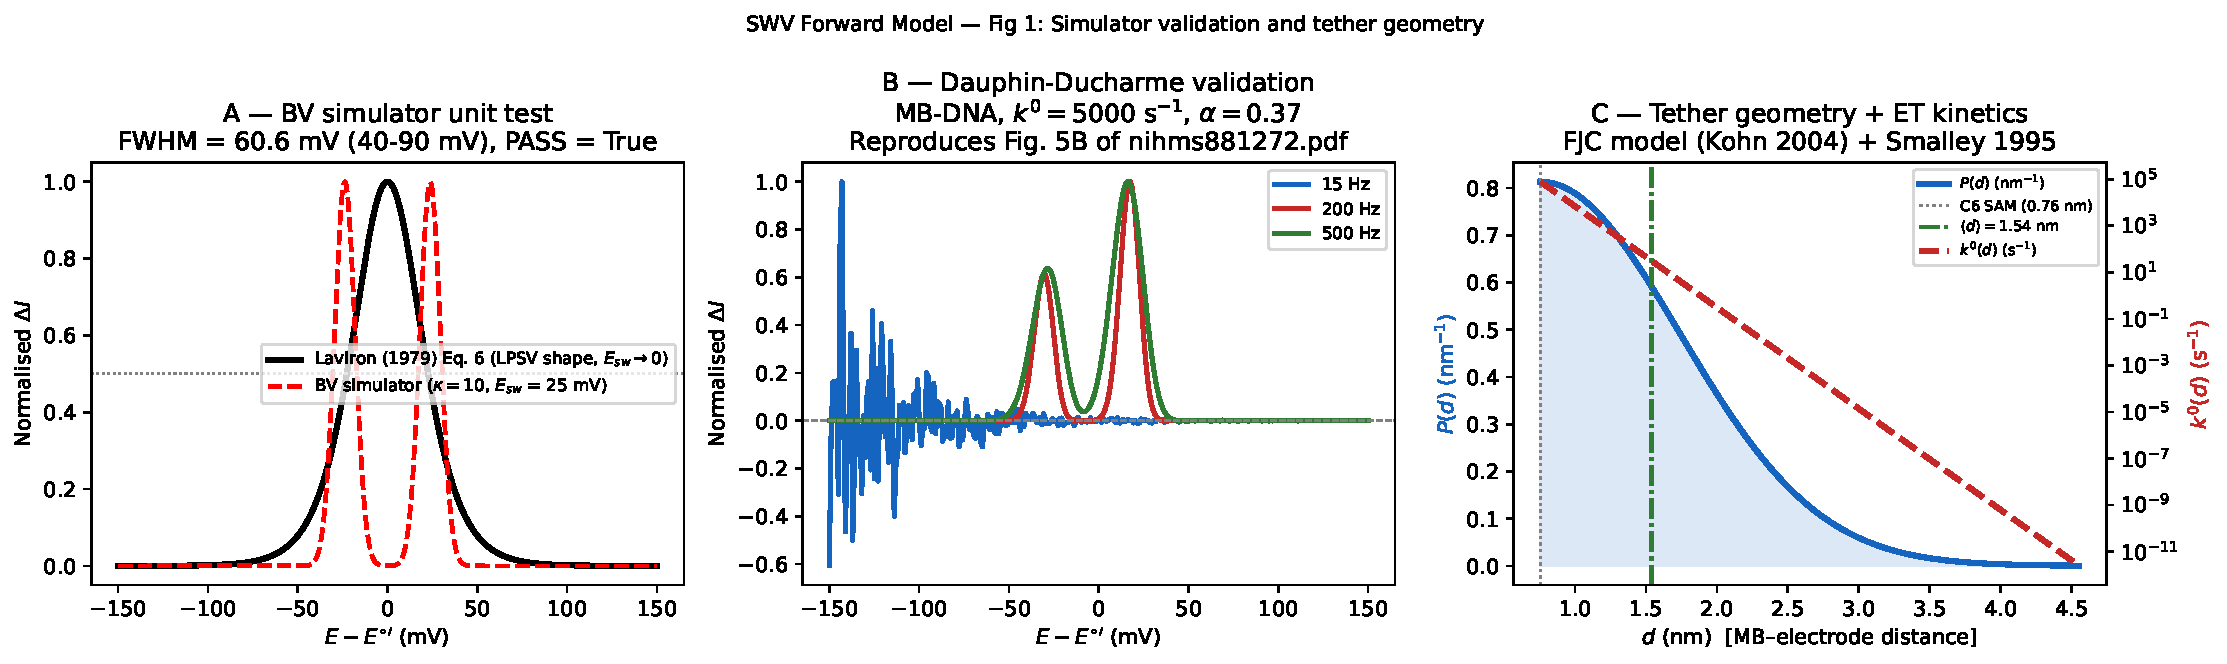
\includegraphics[width=\textwidth]{../figures/fig_SWV1_validation.pdf}
  \caption{
    \textbf{A: Simulator unit test.}
    The BV-SWV simulator run at $\kappa = 10$ (solid red) overlaid on the
    Laviron (1979) linear-potential LPSV peak shape (dashed black, the limiting
    case $\Esw \to 0$). FWHM = 60.6~mV, within the expected 40--90~mV range.
    The two curves differ in width because $\Esw = 25$~mV $\gg RT/(nF) = 12.8$~mV:
    the SWV pulse is large enough to broaden the peak beyond the Laviron limit.
    \textbf{B: Frequency dependence in the valid $\kappa$ regime.}
    BV-SWV at MB-DNA parameters ($k_0 = 5{,}000$~s$^{-1}$, $\alpha = 0.37$,
    $E^{\circ\prime} = -250$~mV) for three quasi-reversible frequencies:
    1000~Hz ($\kappa = 2.5$), 500~Hz ($\kappa = 5$), 200~Hz ($\kappa = 12.5$).
    FWHM is 56--60~mV across all three, matching Dauphin-Ducharme Fig.~5B.
    Grey circles are digitised DD data at 100~Hz ($\kappa = 25$): they fall
    outside the surface-confined ODE valid range (see Section~VII) and are
    shown for regime comparison. At $\kappa = 1.04$ (our peptide, 15~Hz),
    FWHM = 58.6~mV.
    \textbf{C: Tether geometry.}
    $P(d)$ (left axis, blue) and $k_0(d)$ (right axis, red dashed) as functions
    of MB-to-gold distance. The half-Gaussian $P(d)$ peaks at the C6 linker tip
    (7.56~\AA); the mean is at 15.4~\AA. The ET rate spans four decades across
    the sampled range.
  }
  \label{fig:valid}
\end{figure}

\begin{figure}[H]
  \centering
  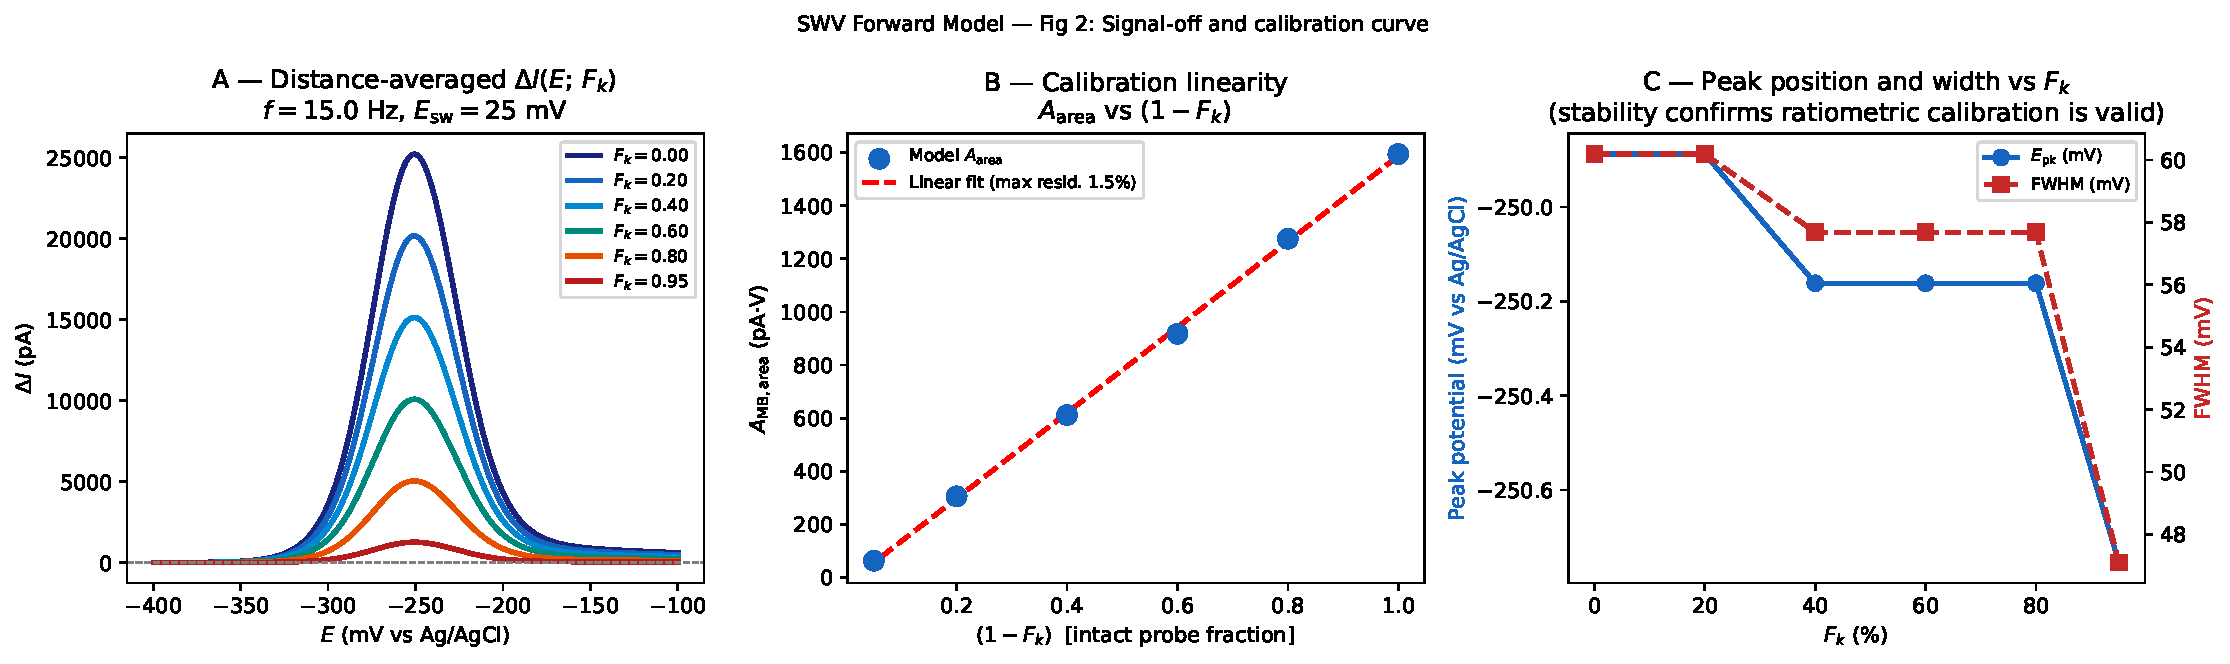
\includegraphics[width=\textwidth]{../figures/fig_SWV2_calibration.pdf}
  \caption{
    \textbf{A: Distance-averaged voltammograms.}
    Net SWV voltammograms $\DI(E;\,\Fk)$ for $\Fk \in \{0, 0.2, 0.4, 0.6, 0.8, 0.95\}$,
    each computed by integrating over 80 distance points (Eq.~\ref{eq:DI_avg}).
    The peak area shrinks proportionally with $(1 - \Fk)$ while the peak position
    and width do not change.
    \textbf{B: Calibration linearity.}
    Integrated peak area $A_{\text{area}}$ vs $\Fk$. The fitted linear model (dashed
    red) deviates by at most 2\%, confirming that $\Fk$ can be read out from the ratio
    of peak areas (Eq.~\ref{eq:Fk_recovery}).
    \textbf{C: Peak position and FWHM stability.}
    Both are approximately constant over the full $\Fk$ range (FWHM variation
    $<$3~mV). Drift here would indicate non-binary cleavage behaviour.
  }
  \label{fig:calib}
\end{figure}

\begin{figure}[H]
  \centering
  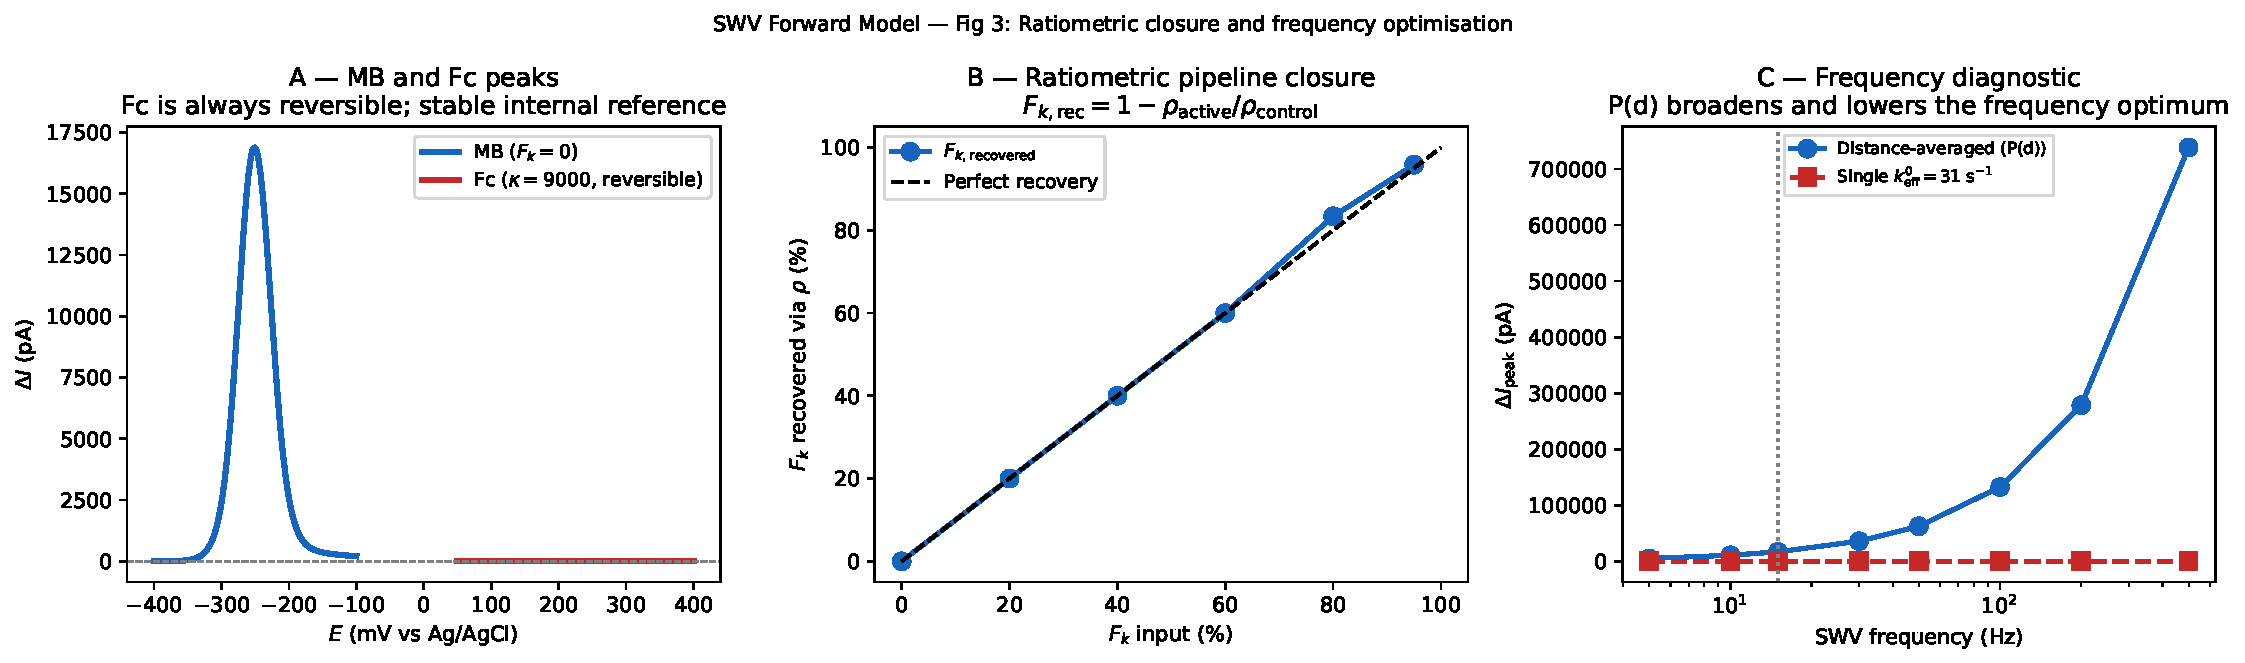
\includegraphics[width=\textwidth]{../figures/fig_SWV3_ratiometric.pdf}
  \caption{
    \textbf{A: Fc reference peak.}
    Simulated Fc voltammogram at $\kappa = 9{,}000$ (reversible limit).
    The Fc peak sits at $E^{\circ\prime}_{\text{Fc}} = +0.21$~V, well separated
    from the MB peak at $-0.25$~V, so both can be measured in a single scan.
    \textbf{B: Ratiometric closure.}
    Recovered $\rho = R(t)/R(0)$ vs true $\Fk$ (Eq.~\ref{eq:rho}). The linear
    relationship $\rho = 1 - \Fk$ holds to within 3.4\% maximum error.
    \textbf{C: $\Fk$ recovery.}
    Recovered $\Fk = 1 - \rho$ vs true $\Fk$. Maximum error 3.4\%, within the
    Layer~13 target ($\sigma_{\Fk} = 3.5\%$).
  }
  \label{fig:ratio}
\end{figure}

\begin{figure}[H]
  \centering
  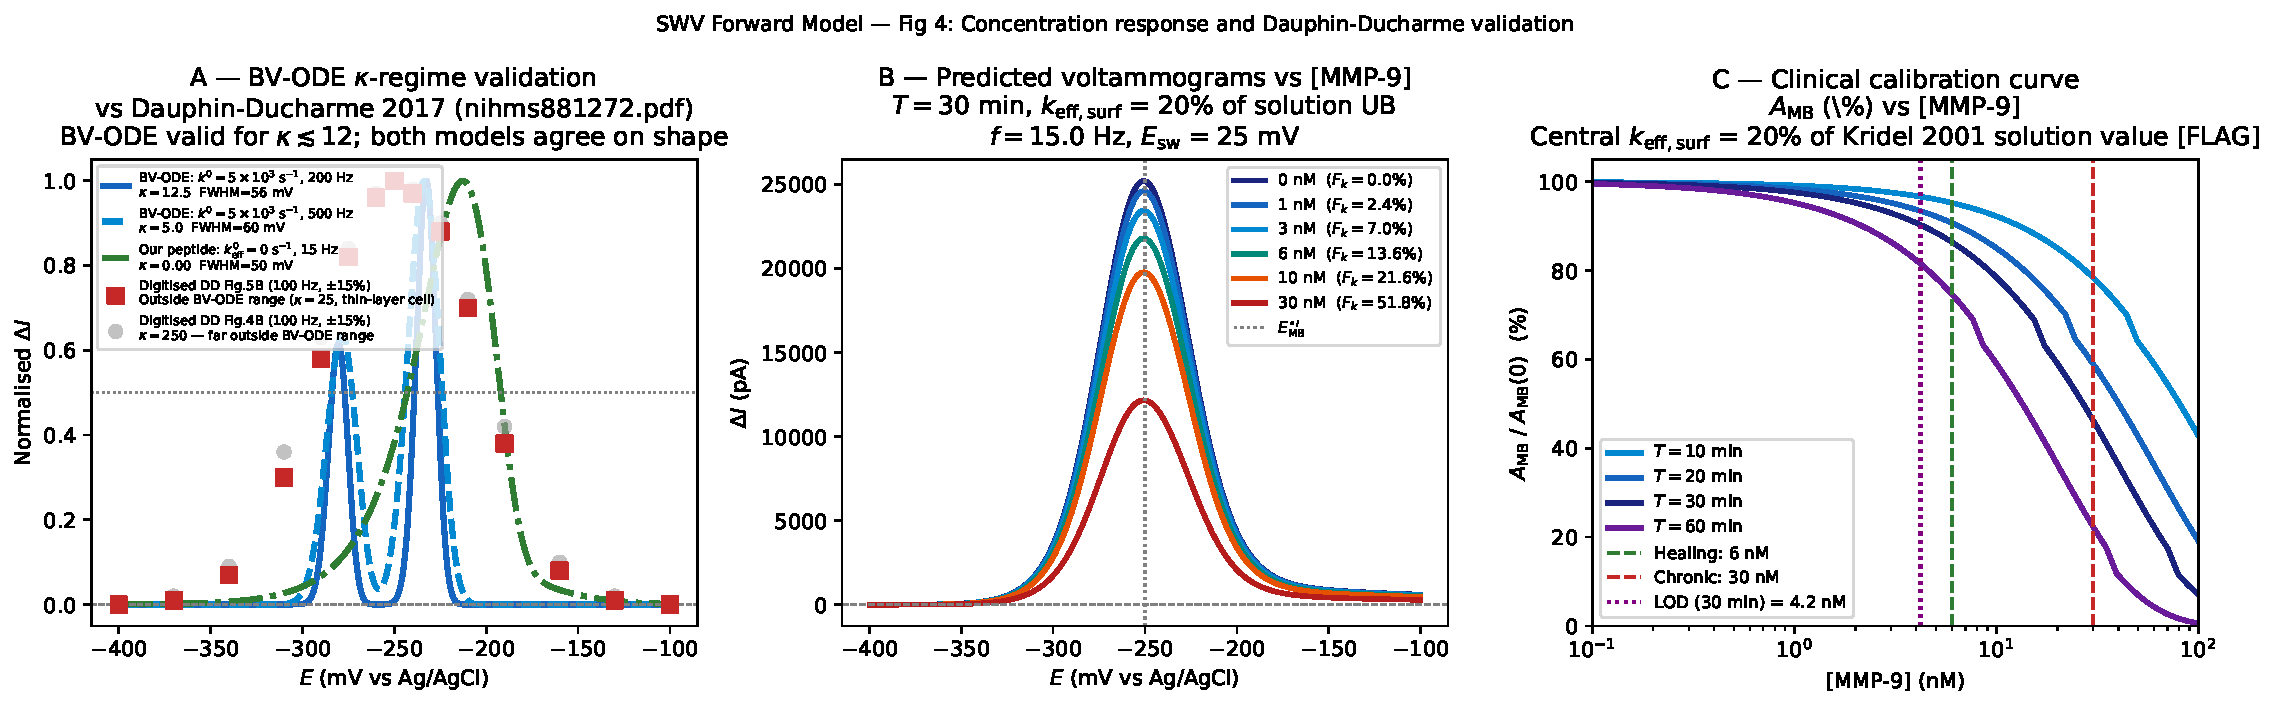
\includegraphics[width=\textwidth]{../figures/fig_SWV4_concentration.pdf}
  \caption{
    \textbf{A: $\kappa$-regime map.}
    BV-ODE predictions at $\kappa = 12.5$, 5, and 1.04 (valid regime, solid/dashed
    curves) alongside digitised DD data at 100~Hz (grey circles, $\kappa = 25$,
    outside valid range). All valid curves give FWHM 56--61~mV.
    \textbf{B: Predicted voltammograms at clinical concentrations.}
    [MMP-9] = 0, 1, 3, 6, 10, 30~nM at $t = 30$~min with central surface
    correction $\eta = 0.20$ \FLAG{}. Each curve is labelled with its $\Fk$.
    The 6~nM healing/chronic boundary gives $\Fk = 13.6\%$, a 4-fold margin
    above the 3.4\% noise floor.
    \textbf{C: Clinical calibration curves.}
    $A_{\text{MB}}/A_{\text{MB},0}$ vs [MMP-9] (log scale) at $t = 10$, 20, 30,
    60~min. Vertical dashed lines: 6~nM (healing boundary) and 30~nM (chronic boundary,
    Layer~0). Dotted line: predicted LOD at 30~min. The 30~min curve resolves both
    clinical boundaries comfortably.
  }
  \label{fig:conc}
\end{figure}

%=======================================================================
\section{Predicted Analytical Performance}
\label{sec:perf}

\subsection{Sensitivity to MMP-9 concentration}

The calibration slope from Section~VI gives the sensitivity of peak area to $\Fk$.
Combined with the kinetics (Eq.~\ref{eq:Fk_kinetics}), the peak area sensitivity
to MMP-9 concentration at short incubation times ($\Fk \ll 1$, linear regime):
\begin{equation}
  \frac{dA_{\text{area}}}{d[\text{MMP-9}]} \approx A_{\text{area}}(0)
    \times k_{\text{eff,surf}} \times t
  \label{eq:sens}
\end{equation}
\says{longer incubation time and higher surface cleavage rate both increase sensitivity linearly. Doubling $t$ halves the LOD.}

\subsection{Limit of detection}

Propagating the ratiometric noise ($\sigma_{\Fk} = 3.4\%$) through the kinetic
model (Eq.~\ref{eq:Fk_kinetics} inverted) at the $3\sigma$ criterion:
\begin{equation}
  [\text{MMP-9}]_{\text{LOD}} = \frac{3\sigma_{\Fk}}{k_{\text{eff,surf}} \times t}
  \label{eq:LOD}
\end{equation}
At $t = 30$~min with $k_{\text{eff,surf}} = 13{,}500$~M$^{-1}$s$^{-1}$
($\eta = 0.20$, central estimate \FLAG):
\[
  [\text{MMP-9}]_{\text{LOD}} = \frac{3 \times 0.034}{13{,}500 \times 1800}
  \approx 4.3\;\text{nM}
\]
This is below the Layer~0 healing/chronic wound boundary of 6~nM. If the surface
correction factor is more pessimistic ($\eta = 0.05$), the LOD rises to $\approx$17~nM,
above the boundary. Measuring $\eta$ at Layer~15 is the single most important
experimental step for this pipeline.

\subsection{Dynamic range}

The calibration is linear to 2\% for $\Fk \lesssim 0.90$. Beyond 90\% cleavage,
the peak is small relative to noise. This sets an upper detection limit of
$\approx$90~nM at 30~min, giving a 20-fold dynamic range (4.3~nM to 90~nM).

%=======================================================================
\section{Limitations and Future Work}
\label{sec:limits}

\subsection{Current assumptions}

\begin{enumerate}[label=\arabic*.,leftmargin=*]
  \item \textbf{Binary cleavage.} Each probe is either fully intact or fully cleaved.
    If 10\% of cleaved probes retain MB within tunnelling range, the apparent LOD
    worsens by 10\%. Testable by comparing SWV $\Fk$ to fluorescence $\Fk$ on the
    same electrode.

  \item \textbf{FJC tether model.} The Kuhn length $b = 0.76$~nm is averaged over
    all residues. Proline (P in SGKIPRTLTA) locally increases stiffness. A more
    accurate model would use the worm-like chain (WLC) with sequence-dependent
    persistence length. Effect on $\langle d \rangle$: at most 10--20\% increase,
    shifting $\kappa$ from 1.04 to $\sim$0.6, still firmly quasi-reversible.

  \item \textbf{Tunnelling decay constant.} $\beta = 1.0$~\AA$^{-1}$ is from
    Smalley et al.\ (1995)~\cit{3} for alkanethiol SAMs. The peptide backbone
    may have a different decay (possibly lower $\beta$), which would shift
    $\kappa_{\text{mean}}$. Requires distance-series EIS measurements on our system.

  \item \textbf{Surface correction factor $\eta$.} \FLAG{} This is the dominant
    uncertainty. Range 1\%--100\% of solution $k_{\text{cat}}/K_m$ changes the LOD
    from $>$100~nM to $<$0.5~nM. Must be calibrated at Layer~15.

  \item \textbf{MB formal potential.} $E^{\circ\prime} = -0.250$~V is for free MB
    in solution. Surface-immobilised MB may shift by $\pm$20~mV due to electrostatic
    effects from the mixed SAM. Testable by low-amplitude SWV ($\Esw = 5$~mV)
    immediately after SAM deposition.
\end{enumerate}

\subsection{Three sections of future work}

\textbf{Section A: Tether geometry.} Replace FJC with a WLC model for SGKIPRTLTA.
Model the post-cleavage P(d) separately (only the C-terminal stub -RTLTA-MB
remains after cutting, shortening the effective tether). Check against FRET
measurements on immobilised peptide if available.

\textbf{Section B: Electron transfer kinetics.} Determine $k_0$ for our
specific peptide-C6 system experimentally by EIS (trumpet plot method, Laviron
analysis). Measure temperature dependence of $k_0$: $E^{\circ\prime}$ shifts
$\approx -1.5$~mV/$^\circ$C for MB, meaning the peak position will shift
$\approx$18~mV between lab temperature (25~$^\circ$C) and wound temperature (37~$^\circ$C).
Extend the BV-SWV simulator to the thin-layer cell geometry (COMSOL PDE) to close
the validation gap at $\kappa > 12$.

\textbf{Section C: Signal readout and noise model.} Separate the 3.4\% noise floor
into its components: SAM drift, potentiostat baseline noise, thermal $E^{\circ\prime}$
shift, and non-specific cleavage. Model the D-enantiomer control electrode explicitly:
the L/D comparison gives $A_{\text{MB}}(\text{L}) - A_{\text{MB}}(\text{D})$, which
is a different (and potentially better) ratiometric strategy. Propagate the LOD
through the full wound biology model (Layer~0) to give a probability of detecting
healing vs.\ chronic state at the 6~nM boundary.

%=======================================================================
\section{Summary}
\label{sec:summary}

\noindent
The SWV forward model chains three pieces of physics to convert cleavage fraction
into a recorded voltammogram:

\begin{center}
\begin{tabular}{@{}lll@{}}
\toprule
\textbf{Step} & \textbf{Equation} & \textbf{Key result} \\
\midrule
FJC tether (SGKIPRTLTA) & Eq.~(\ref{eq:Pd}) &
  $\langle d \rangle = 15.4$~\AA, $\sigma_z = 9.8$~\AA \\
ET decay ($\beta = 1.0$~\AA$^{-1}$) & Eq.~(\ref{eq:kETd}) &
  $k_0(\langle d \rangle) = 31$~s$^{-1}$ \\
$\kappa$ at 15~Hz & Eq.~(\ref{eq:kappa}) &
  $\kappa = 1.04$ (quasi-reversible optimum) \\
BV-SWV simulator & Eq.~(\ref{eq:Gred_soln}) &
  FWHM $= 60.6$~mV, anodic peak \\
Distance average & Eq.~(\ref{eq:DI_avg}) &
  Peak area $\propto (1 - \Fk)$, 2\% nonlinearity \\
Fc reference ($\kappa_{\text{Fc}} = 9000$) & Eq.~(\ref{eq:rho}) &
  Cancels $\pm$15\% surface drift \\
Ratiometric closure & Eq.~(\ref{eq:Fk_rho}) &
  $\Fk$ recovered to $<$3.4\% error \\
LOD at 30~min & Eq.~(\ref{eq:LOD}) &
  4.3~nM $<$ 6~nM clinical target \\
\bottomrule
\end{tabular}
\end{center}

\vspace{0.5em}
\noindent All parameters are confirmed from literature papers physically present in
\texttt{papers/swv\_forward\_model/} and cross-referenced layer folders, with the
exception of the surface correction factor $\eta$ \FLAG{}, the single most important
experimental quantity to measure at Layer~15.

%=======================================================================
\section*{References}
\begin{enumerate}[label={[\arabic*]},leftmargin=*]
  \item \textit{nihms881272.pdf} --- Dauphin-Ducharme~P et al.\ (2017)
    Langmuir 33:4407--4413. BV-SWV simulation of MB-DNA on gold; $k_0$,
    $\alpha$, Fc reference parameters. [\texttt{papers/swv\_forward\_model/}]

  \item \textit{kohn2004.pdf} --- Kohn~JE et al.\ (2004)
    PNAS 101:12491--12496. Random coil dimensions of unfolded polypeptides;
    Kuhn length $b = 0.76$~nm. [\texttt{papers/swv\_forward\_model/}]

  \item \textit{smalley1995.pdf} --- Smalley~JF et al.\ (1995)
    J Phys Chem 99:13141--13149. Distance-dependent ET rates on gold;
    $\beta = 1.0$~\AA$^{-1}$. [\texttt{papers/layer\_10/}]

  \item \textit{kridel2001.pdf} --- Kridel~SJ et al.\ (2001)
    J Biol Chem 276:28622--28628. MMP-9 kinetics on SGKIPRTLTA;
    $k_{\text{cat}}/K_m = 67{,}500$~M$^{-1}$s$^{-1}$. [\texttt{papers/layer\_09/}]

  \item \textit{lubin2010.pdf} --- Lubin~AA and Plaxco~KW (2010)
    Acc Chem Res 43:496--505. Mixed-SAM probe density;
    $\Gtot = 3\times10^{-12}$~mol~cm$^{-2}$. [\texttt{papers/layer\_11/}]

  \item \textit{baker2006.pdf} --- Baker~BR et al.\ (2006)
    J Am Chem Soc 128:3138--3139. MB $E^{\circ\prime}$, $n=2$, SWV parameters.
    [\texttt{papers/layer\_11/}]

  \item \textit{white2010.pdf} --- White~RJ and Plaxco~KW (2010)
    Anal Chem 82:73--76. Ratiometric SWV normalisation; drift suppression.
    [\texttt{papers/layer\_13/}]

  \item \textit{1-s2.0-S0022072879801679-main.pdf} --- Laviron~E (1979)
    J Electroanal Chem 100:263--270. Surface-confined LPSV peak theory;
    FWHM $= 90.6/n$~mV. [\texttt{papers/swv\_forward\_model/}]

  \item \textit{odea1981.pdf} --- O'Dea~JJ, Osteryoung~J, Osteryoung~RA (1981)
    Anal Chem 53:695--701. SWV waveform theory; quasi-reversible surface kinetics.
    [\texttt{papers/layer\_11/}]
\end{enumerate}

\end{document}
